\documentclass{article}
\usepackage[utf8]{inputenc}
\usepackage[T1]{fontenc}
\usepackage[portuguese]{babel}

\usepackage{indentfirst}
\usepackage{makeidx}
\usepackage{stackengine}
\usepackage{amssymb}
\usepackage{amsthm}
\usepackage{hyperref}
\usepackage{color}
\usepackage{graphicx}


\title{\bf{Aprendizagem Computacional - Trabalho Prático 2}\vspace{80mm}}
\author{\textbf{João Tiago Márcia do Nascimento Fernandes - 2011162899} \\
\textbf{Joaquim Pedro Bento Gonçalves Pratas Leitão - 2011150072}}
\makeindex

\begin{document}

\maketitle

\pagebreak

\renewcommand*\contentsname{Índice}
\tableofcontents

\pagebreak

\section{Introdução}

Este trabalho foca-se no reconhecimento de caracteres da numeração árabe, ou seja, os caracteres 0 a 9.

Pretende-se que este reconhecimento seja realizado por uma aplicação desenvolvida em \emph{Matlab}, que faz uso de redes neuronais na sua arquitetura interna, disponíveis na \emph{Nerual Networks Toolbox} do próprio \emph{Matlab}.

A aplicação desenvolvida visa o estudo de duas arquiteturas distintas no reconhecimento dos caracteres:

\begin{itemize}
\item Na primeira arquitetura a aplicação será constituída por uma \emph{memória associativa} e um \emph{classificador}

\item Na segunda arquitetura a aplicação apenas recorre ao \emph{classificador}
\end{itemize}

\vspace{.3cm}

As duas arquiteturas apresentadas estão presentes nas figuras que se seguem:

\begin{figure}[h]
  \centering
      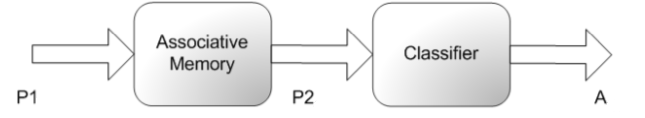
\includegraphics[scale=0.4]{AM_Classifier.png}
  \caption{Arquitetura da aplicação com \emph{memória associativa + classificador}}
\end{figure}

\begin{figure}[h]
  \centering
      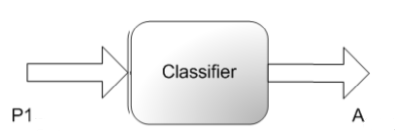
\includegraphics[scale=0.4]{Classifier.png}
  \caption{Arquitetura da aplicação apenas com o \emph{classificador}}
\end{figure}

Através da análise destas figuras podemos determinar um comportamento padrão para a aplicação:

\begin{itemize}
\item Numa fase inicial, os caracteres a identificar poderão, ou não, ser fornecidos à \emph{memória associativa}, que está encarregue da sua "filtragem" ou "correção": Se os caracteres fornecidos não forem perfeitos, a memória associativa aproxima-os dos respetivos caracteres perfeitos.

\item De seguida os dados, corrigidos ou não, serão fornecidos ao \emph{classificador}, que se encarregará de proceder à identificação dos mesmos.
\end{itemize}

No presente documento iremos proceder à apresentação em maior detalhe destas duas arquiteturas e das suas implementações, bem como da aplicação \emph{Matlab} desenvolvida, e de como poderá ser utilizada. Pretendemos também fazer uma análise crítica da performance da aplicação, nomeadamente da sua capacidade de classificar corretamente novos caracteres fornecidos.

\pagebreak

\section{Aplicação Desenvolvida}

A aplicação desenvolvida visa identificar corretamente caracteres desenhados pelo utilizador, implementando para isso as duas arquiteturas apresentadas anteriormente: \emph{Memória Associativa + Classificador} e \emph{Classificador}.

Ambas as arquiteturas e os respetivos modos de funcionamento serão apresentados de seguida.

\subsection{Memória Associativa + Classificador}

Na arquitetura \emph{Memória Associativa + Classificador}, os dados 

\subsection{Classificador}

\pagebreak

\subsection{Implementação em Matlab}

Para o desenvolvimento da aplicação foi-nos fornecido código-fonte, que cria e disponibiliza ao utilizador uma grelha onde este irá desenhar os caracteres a identificar, encarregando-se de toda a lógica interna da aplicação com a exceção da implementação do sistema de classificação dos caracteres e de toda a lógica a ele inerente (implementação das diferentes arquiteturas da aplicação, realização dos treinos das redes neuronais implementadas, etc)

\subsubsection{associativeMemory.m}


\subsubsection{createNetwork.m}


\subsubsection{myclassify.m}


\subsubsection{run.m}

Este é o ficheiro a executar para que a aplicação possa ser testada e utilizada.

\subsection{Execução}

Para executar a aplicação o utilizador deverá executar o ficheiro \emph{run.m}. Uma vez iniciado, será pedido ao utilizador que selecione uma de duas possíveis arquiteturas para a aplicação: Utilizando \emph{Memória Associativa} em conjunto com o \emph{Classificador}, e utilizando apenas o \emph{Classificador}.

Caso o utilizador selecione a utilização da \emph{Memória Associativa}, então terá de escolher o tipo de treino a realizar na mesma.

Existem dois tipos de treino distintos: O primeiro recorre à \emph{Pseudo-Inversa}, onde os pesos da rede neuronal que a \emph{Memória Associativa} implementa são calculados pelo produto do \emph{output} esperado pelo valor da aplicação função \emph{pinv} (nativa do \emph{Matlab}) aos dados de \emph{input}. Já o segundo faz uso da \emph{Regra de Hebb} para calcular os pesos: Aqui os pesos resultam do produto do \emph{output} esperado pela seguinte matriz: $input^{T}\times \left(input\times input^{T}\right)^{-1}$.

Após esta seleção a \emph{Memória Associativa} é criada, aparecendo de seguida uma grelha, onde o utilizador desenhará os caracteres a serem classificados. Assim que os caracteres são desenhados, o utilizador tem de carregar no botão do meio do seu rato, de forma a transitar para a fase de execução seguinte.

Nesta fase, o utilizador terá que escolher algumas características da rede neural que o classificador da aplicação implementa. Caso já exista alguma rede previamente criada com as características especificadas pelo utilizador, essa rede é carregada para memória e utilizada na execução. Caso ainda não exista, uma rede neuronal com as características desejadas é criada e treinada, sendo também guardada para posteriores execuções. 

Uma vez obtida a rede a utilizar, esta classifica os dados introduzidos pelo utilizador, que lhe serão apresentados numa grelha semelhante à onde inicialmente desenhou os caracteres.


\pagebreak

\section{Testes e Resultados}

Descrição de como fizémos os casos de teste, dimensões, etc

\pagebreak

\section{Conclusões}

Conclusões, lolol

\pagebreak

\textbf{FIXME: Testar classificação de dígitos perfeitos e de dígitos não perfeitos (alguns não perfeitos são corretamente classificados, e todos os perfeitos são corretamente classificados)}

\textbf{FIXME: Dizer que memória associativa só funciona se preenchermos a tabela toda pela ordem: 1,2,3,4,5,6,7,8,9,0 linha-a-linha}

\vspace{.3cm}

\textbf{FIXME: Perguntas relatório:}

\begin{itemize}
\item How does the data set influence the performance of the classification system?

\item Which architecture provides better results: only the classifier or the associative memory+classifier?

\item Which is the best activation function: hardlim, linear or logsig?

\item Does the Hebb rule perform well?

\item Is the classification system able to achieve the main objectives (classification of digits)?

\item Which is the percentage of well classified digits?

\item How is the generalization capacity?

\item Is the classification system robust enough to give correct outputs when new inputs are not perfect?

\item Which is the percentage of well classified new inputs?
\end{itemize}

\pagebreak

\end{document}